\documentclass[10pt,pdf,hyperref={unicode}]{beamer}

\mode<presentation>
{
\usetheme{boxes}
\beamertemplatenavigationsymbolsempty

\setbeamertemplate{footline}[page number]
\setbeamersize{text margin left=0.5em, text margin right=0.5em}
}

\usepackage[utf8]{inputenc}
\usepackage[english, russian]{babel}
\usepackage{bm}
\usepackage{multirow}
\usepackage{ragged2e}
\usepackage{indentfirst}
\usepackage{multicol}
\usepackage{subfig}
\usepackage{amsmath,amssymb}
\usepackage{enumerate}
\usepackage{mathtools}
\usepackage{comment}
\usepackage{multicol}
\usepackage{color}
\definecolor{python-green}{RGB}{55,126,33}

\usepackage[all]{xy}

\usepackage{tikz}
\usetikzlibrary{positioning,arrows}

\tikzstyle{name} = [parameters]
\definecolor{name}{rgb}{0.5,0.5,0.5}

\usepackage{caption}
\captionsetup{skip=0pt,belowskip=0pt}

\newtheorem{rustheorem}{Теорема}
\newtheorem{russtatement}{Утверждение}
\newtheorem{rusdefinition}{Определение}

% colors
\definecolor{darkgreen}{rgb}{0.0, 0.2, 0.13}
\definecolor{darkcyan}{rgb}{0.0, 0.55, 0.55}

\AtBeginEnvironment{figure}{\setcounter{subfigure}{0}}%

\captionsetup[subfloat]{labelformat=empty}

%----------------------------------------------------------------------------------------------------------

\title[Априорное распределение параметров в задачах выбора моделей глубокого обучения]{Априорное распределение параметров \\в задачах выбора моделей глубокого обучения}
\author{А.\,В.\,Грабовой}

\institute[]{Диссертация на соискание ученой степени\\
кандидата физико-математических наук\\05.13.17~--- Теоретические основы информатики\\Научный руководитель: д.ф.-м.н. В.\,В. Стрижов\\}
\date[2022]{\small 21\;апреля\;2022\,г.}

%---------------------------------------------------------------------------------------------------------
\begin{document}

\begin{frame}
\titlepage
\end{frame}

%----------------------------------------------------------------------------------------------------------
\section{Априорное распределение параметров моделей}
\begin{frame}{Априорное распределение параметров моделей}
\bigskip
\justifying
Исследуется проблема выбора моделей глубокого обучения. Для выбора моделей используется связный байесовский вывод. Для снижения размерности пространства параметров при выборе модели используется информация об их априорном и апостериорном распределениях.
\begin{block}{Цель исследования~---}
\justifying
предложить метод задания априорного распределения параметров модели глубокого обучения с учетом накопленной информации о решаемой задаче.
\end{block}
\begin{block}{Требуется предложить}
\justifying
метод выбора модели, основанный на использовании привилегированной и накопленной информации, выравнивания структур параметрических моделей для снижения размерности пространства параметров моделей.
\end{block}
\begin{block}{Практическая ценность}
\justifying
Снижение размерности пространства параметров моделей глубокого обучения при незначительной потере качества позволяет использовать модели глубокого обучения на устройствах с низкой производительностью, в частности, на мобильных устройствах.
\end{block}
\end{frame}
%---------------------------------------------------------------------------------------------------------
\section{Привилегированное обучение Вапника и Хинтона}
\begin{frame}{Привилегированное обучение {\color{red}В.\,Н.\;Вапника\footnotemark} и \\ \hfill\hfill\hfill\hfill\hfill дистилляция~{\color{blue}Дж.\;Хинтона\footnotemark}}
%\justifying
Заданы
\begin{enumerate}[1)]
    \item признаки~$\mathbf{x}_i \in \mathbb{R}^{n}$ и привилегированные признаки~$\mathbf{x}^*_i \in \mathbb{R}^{n^*}$,
    \item целевая переменная~$y_i \in \mathbb{Y}$,
    \item индексы объектов, для которых известна привилегированная информация $\mathcal{I},$ а для которых она не известна $\bar{\mathcal{I}}$.
\end{enumerate}

Модели учителя~$\mathbf{f}:\mathbb{R}^{n^*} \to \mathbb{Y}^\prime$ и ученика~$\mathbf{g}:\mathbb{R}^{n} \to \mathbb{Y}^\prime$~--- пространство оценок.

Ответы $\mathbf{s}_i = \mathbf{f}\bigr(\mathbf{x}_i^*\bigr)$ функции $\mathbf{f}$ для объектов~$\mathbf{x}^*_i$.

\bigskip

Требуется выбрать модель ученика~$\mathbf{g}$ из множества
\[
	\mathfrak{G} = \left\{\mathbf{g}| \mathbf{g}:\mathbb{R}^{n} \to \mathbb{Y}^\prime\right\}.
\]
Оптимизационная задача:
\[
	\mathbf{g} = \arg\min_{\mathbf{g} \in \mathfrak{G}} \mathcal{L}\bigr(\mathbf{g}, \mathbf{f}, \mathbf{X}, \mathbf{X}^{*}, \mathbf{y},\mathbf{s}\bigr),
\]
где $\mathcal{L}$~--- функция ошибки.

\bigskip
\footnotetext[1]{\textit{Lopez-Paz D., Bottou L., Scholkopf B., Vapnik V.} {\color{red}Unifying distillation and privileged information} // ICLR, 2016.}
\footnotetext[2]{\textit{Hinton G., Vinyals O., Dean J.} {\color{blue}Distilling the knowledge in a neural network} // NIPS, 2015.}
\end{frame}

%---------------------------------------------------------------------------------------------------------
\section{ФРЕЙМЫ}
\begin{frame}
\frametitle{Байесовская дистилляция модели}

\begin{minipage}[t][4.1cm][t]{\textwidth}
~\\[-2mm]
\begin{equation*}
\xymatrix{
% First Line
\parbox{3em}{
\footnotesize Задача \\ оптимизации
}
&
\parbox{3em}{
\centering
$\hat{\mathbf{w}}, \hat{\mathbf{A}}_{w}\ar[r]^{g}$
}
& 
\hat{y}\ar[rr]
&
\parbox{3em}{
\centering
}
& 
\parbox{10em}{
\centering
$
{\mathcal{L}\bigr(\mathbf{w},\mathbf{A}_{\text{w}}|{\color{blue} s, }y, \hat{y}, {\color{python-green}\mathbf{w}_0, \mathbf{A}_0}\bigr)}
\ar@/_2pc/[lll]
$
}
\\
% Second Line
{
\parbox{3em}{\footnotesize Дополнительная \\ информация}
}
&
{\mathfrak{G} \ar[u]}
&
{\color{blue} s \ar@[blue][urr]}
&
{ \hat{\mathbf{u}}, \hat{\mathbf{A}}_{ \text{u}} \ar@[python-green][r] \ar[l]^{f}}
&
{\color{python-green} \left(\mathbf{w}_0, \mathbf{A}_0\right) \ar[u]}
\\
% Third Line
\parbox{3em}{\footnotesize Выборка}
&
&
\parbox{3em}{
\centering
$
$
}
& 
{\left(\mathbf{x}, y\right) \ar@{.>}[uul] \ar@{.>}[uur] \ar@{.>}[ul]}
&
}
\end{equation*}
\end{minipage}

\vfill
\vspace{0.5cm}
\begin{itemize}
\item[] Выборка
    {
        $\mathfrak{D}\ni(\mathbf{x},y)$,
        $\quad \mathbf{x} \in \mathbb{R}^{n}, y \in \mathbb{Y}$ 
    }
    \item[] Ученик $\mathfrak{G}\ni\mathbf{g}: \mathbb{R}^{n}\times\mathbb{R}^{n_{w}} \to \mathbb{Y}^\prime$
        {
            $\quad\text{и учитель~}{\mathbf{f}:\mathbb{R}^{n}\times \mathbb{R}^{n_{w}} \to \mathbb{Y}^\prime}$
        }
    \item[] Прогноз $\hat{y} = g\bigr(\mathbf{x}, \hat{\mathbf{w}})$
        {
            $\quad \text{и~}
            {\color{blue} s = f\bigr(\mathbf{x}, \hat{\mathbf{u}})}$}
    \item[] Априорное распределение 
        {
            $\mathbf{w} \sim \mathcal{N}\bigr({\color{python-green}\mathbf{w}_0\bigr(\hat{\mathbf{u}}, \hat{\mathbf{A}}_{\text{u}}\bigr)}, {\color{python-green}\mathbf{A}_0\bigr(\hat{\mathbf{u}}, \hat{\mathbf{A}}_{\text{u}}\bigr)}\bigr)$.
        }
    \item[] Оптимизационная задача
        {
            \[
            \hat{\mathbf{w}}, \hat{\mathbf{A}}_{w} = \mathop{\arg\min}_{\mathbf{w} \in \mathbb{R}^{n_{w}}, \mathbf{A} \in \mathbb{R}^{n_{w}\times n_{w}}} \mathcal{L}\bigr(\mathbf{w},\mathbf{A}_{\text{w}}|{\color{blue} \mathbf{s}}, \mathfrak{D}, \mathbf{g},{\mathbf{f}},{\color{python-green}\mathbf{w}_0}, {\color{python-green}\mathbf{A}_0}\bigr)
            \]}
\end{itemize}
\end{frame}

%----------------------------------------------------------------------------------------------------------
\section{Оптимизация модели ученика на основе учителя~и привилегированных признаков}
\begin{frame}{Оптимизация модели ученика на основе учителя~и привилегированных признаков}
~\\[-1mm]
Заданы
\begin{enumerate}[1)]
	\item признаки $\mathbf{x}_i\in \mathbb{R},$
	\item $y_i \in \mathbb{Y}=\{1, \cdots, K\}, \quad \mathbb{Y}^\prime=\mathbb{R}^{K}$.
\end{enumerate}

\medskip
Параметрические семейства учителя и ученика:
\[
\setlength\abovedisplayskip{0pt}
\mathfrak{F}_{\text{cl}} = \left\{\mathbf{f}| \mathbf{f} = \text{softmax}\bigr(\mathbf{v}\bigr(\mathbf{x}\bigr)/T\bigr), \quad \mathbf{v}: \mathbb{R}^{n} \to \mathbb{R}^K \right\},
%\setlength\belowdisplayskip{0pt}
\]
\[
%\setlength\abovedisplayskip{0pt}
\mathfrak{G}_{\text{cl}} = \left\{\mathbf{g}| \mathbf{g} = \text{softmax}\bigr(\mathbf{z}\bigr(\mathbf{x}\bigr)/T\bigr), \quad \mathbf{z}: \mathbb{R}^n \to \mathbb{R}^K \right\},
%\setlength\belowdisplayskip{0pt}
\]
где~$\mathbf{z},\mathbf{v}$~--- дифференцируемые по параметрам функции заданной структуры, $T$~--- параметр температуры.

\medskip
Функция ошибки
\[
\setlength\abovedisplayskip{0pt}
\begin{aligned}
   \mathcal{L}\bigr(\mathbf{g}\bigr) = &-\sum_{i=1}^{m}\underbrace{{\sum_{k=1}^{K}y^k_i\log{g_k}\bigr(\mathbf{x}_i\bigr)\bigr|_{T=1}}}_{\text{исходная функция потерь}}- \sum_{i=1}^{m}\underbrace{{\sum_{k=1}^{K}{f_k}\bigr(\mathbf{x}_i\bigr)\bigr|_{T=T_0}\log{g_k}\bigr(\mathbf{x}_i\bigr)\bigr|_{T=T_0}}}_{\text{слагаемое дистилляции}},
\end{aligned}
\setlength\belowdisplayskip{0pt}
\]
где~$\cdot\bigr|_{T=t}$ фиксирует температуру~$T$.

Оптимальная модель выбирается из класса,
$\hat{\mathbf{g}} = \arg\min\limits_{\mathbf{g} \in \mathfrak{G}_{\text{cl}}} \mathcal{L}\bigr(\mathbf{g}\bigr).$
\end{frame}
%----------------------------------------------------------------------------------------------------------
\section{Вероятностная постановка задачи дистилляции}
\begin{frame}{Вероятностная постановка задачи дистилляции}
\bigskip
\begin{columns}
\column{0.6\textwidth} 
Гипотеза порождения данных:
\begin{enumerate}
	\item[1)] распределение целевой переменной~$p\bigr(y_i|\mathbf{x}_i, \mathbf{g}\bigr)$,
	\item[2)] совместное распределение~$p\bigr(y_i, \mathbf{s}_i|\mathbf{x}_i, \mathbf{g}\bigr)$,
	\item[3)] для всех $i \in \mathcal{I}$ элементы $y_i$ и $\mathbf{s}_i$ являются зависимыми величинами,
	\item[4)] если $|\mathcal{I}|=0$ то решение равно решению максимума правдоподобия.
\end{enumerate}
\column{0.4\textwidth}
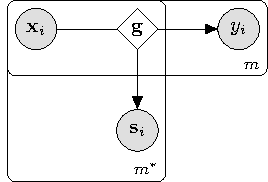
\includegraphics[width=\textwidth]{figures/proba_model}
\end{columns}

\bigskip
Совместное правдоподобие истинных меток и меток учителя:
\[
\setlength\abovedisplayskip{0pt}
p\bigr(\mathbf{y}, \mathbf{S}|\mathbf{X}, \mathbf{g}, \mathcal{I}\bigr)=\prod_{i\not\in \mathcal{I}}p\bigr(y_i|\mathbf{x}_i, \mathbf{g}\bigr)\prod_{i\in \mathcal{I}}p\bigr(y_i, \mathbf{s}_i|\mathbf{x}_i, \mathbf{g}\bigr).
\setlength\belowdisplayskip{0pt}
\]

Задача оптимизации
\[
\setlength\abovedisplayskip{0pt}
\mathbf{g} = \arg\max_{\mathbf{g} \in \mathfrak{G}} p\bigr(\mathbf{y},  \mathbf{S}|\mathbf{X}, \mathbf{g}, \mathcal{I}\bigr),
\setlength\belowdisplayskip{0pt}
\]
имеет вид
\[
\begin{aligned}
\sum_{i\not\in \mathcal{I}}\log p\bigr(y_i|\mathbf{x}_i, \mathbf{g}\bigr) &+ \left(1-\lambda\right)\sum_{i\in \mathcal{I}}\log p\bigr(y_i|\mathbf{x}_i, \mathbf{g}\bigr) + \lambda\sum_{i\in \mathcal{I}}\log p\bigr(\mathbf{s}_i|\mathbf{x}_i, \mathbf{g}\bigr).
\end{aligned}
\]
\end{frame}

%----------------------------------------------------------------------------------------------------------
\section{Вероятностная постановка задачи классификации}
\begin{frame}{Вероятностная постановка задачи классификации}
Заданы
\begin{enumerate}
	\item[1)] учитель $\mathbf{f}\in\mathfrak{F}_{\text{cl}}$ и ученик~$\mathbf{g}\in\mathfrak{G}_{\text{cl}}$,
	\item[2)] распределение истинных меток~$p\bigr(y|\mathbf{x}, \mathbf{g}\bigr) = \text{Cat}\bigr(\mathbf{g}\bigr(\mathbf{x}\bigr)\bigr)$,
	\item[3)] распределение ответов учителя~$p\bigr(\mathbf{s}|\mathbf{x}, \mathbf{g}\bigr) = C\prod_{k=1}^{K}g_k\bigr(\mathbf{x}\bigr)^{s^k}, \quad C < \infty,$
\end{enumerate}
\[
\setlength\abovedisplayskip{0pt}
\begin{aligned}
&\hat{\mathbf{g}} = \arg\max_{\mathbf{g}\in \mathfrak{G}} \sum_{i\not\in \mathcal{I}}\sum_{k=1}^{K}y_i^k\log g_k\bigr(\mathbf{x}_i\bigr)\bigr|_{T=1} 
+ \left(1-\lambda\right)\sum_{i\in \mathcal{I}}\sum_{k=1}^{K}y_i^k\log g_k\bigr(\mathbf{x}_i\bigr)\bigr|_{T=1} +\\
&+ \lambda\sum_{i\in \mathcal{I}}\sum_{k=1}^{K}s_{i,k}\log g_k\bigr(\mathbf{x}_i\bigr)\bigr|_{T=T_0} 
+ \lambda \sum_{i\in \mathcal{I}}\sum_{k=1}^{K}\left(\log g_k\bigr(\mathbf{x}_i\bigr)\bigr|_{T=T_0} + \log\log\frac{1}{g_k\bigr(\mathbf{x}_i\bigr)}\bigr|_{T=T_0}\right).
\end{aligned}
\setlength\belowdisplayskip{0pt}
\]

\begin{rustheorem}[Грабовой, 2020]
\justifying
\label{theorem:st:dist}
Пусть всех $k$ выполняется $1 > 1- \varepsilon > g_k\bigr(\mathbf{x}\bigr) > \varepsilon > 0,$ тогда при
\[
\setlength\abovedisplayskip{0pt}
C=\left(-1\right)^{K}\frac{K^{K/2}}{2^{K(K-1)/2}}\prod_{k=1}^{K}g_k\bigr(\mathbf{x}\bigr)\log g_k\bigr(\mathbf{x}\bigr)
\setlength\belowdisplayskip{0pt}
\]
функция $p\bigr(\mathbf{s}|\mathbf{x}, \mathbf{g}\bigr) = C\prod_{k=1}^{K}g_k\bigr(\mathbf{x}\bigr)^{s^k}$ является плотностью распределения.
\end{rustheorem}

\end{frame}
%----------------------------------------------------------------------------------------------------------
\section{Вероятностная постановка задачи регрессии}
\begin{frame}{Вероятностная постановка задачи регрессии}
Заданы
\begin{enumerate}[1)]
	\item учитель~$f\in\mathfrak{F}_{\text{rg}}= \left\{f| f = \mathbf{v}\bigr(\mathbf{x}\bigr), \quad \mathbf{v}: \mathbb{R}^{n} \to \mathbb{R} \right\}$,
	\item ученик~$g\in\mathfrak{G}_{\text{rg}} = \left\{g| g = \mathbf{z}\bigr(\mathbf{x}\bigr), \quad \mathbf{z}: \mathbb{R}^n \to \mathbb{R} \right\}$,
	\item распределение истинных меток $p\bigr(y|\mathbf{x}, g\bigr) = \mathcal{N}\bigr(y|g\bigr(\mathbf{x}\bigr), \sigma\bigr)$,
	\item распределения меток учителя $p\bigr(s| \mathbf{x}, g\bigr) = \mathcal{N}\bigr(s|g\bigr(\mathbf{x}\bigr), \sigma_s\bigr).$
\end{enumerate}
Оптимизационная задача:
\[
\setlength\abovedisplayskip{0pt}
\begin{aligned}
\hat{g} = \arg\min_{g\in \mathfrak{G}} & \sum_{i\not\in \mathcal{I}}\sigma^2\left(y_i-g\bigr(\mathbf{x}_i\bigr)\right)^2 + \\
&+ \left(1-\lambda\right)\sum_{i\in \mathcal{I}}\sigma^2\left(y_i-g\bigr(\mathbf{x}_i\bigr)\right)^2 + \lambda\sum_{i\in \mathcal{I}}\sigma_s^2\left(s_i-g\bigr(\mathbf{x}_i\bigr)\right)^2.
\end{aligned}
\setlength\belowdisplayskip{0pt}
\]

\begin{rustheorem}[Грабовой, 2020]
\justifying
\label{theorem:st:reg}
Пусть~$\mathfrak{G}_{rg}$ --- класс линейных функций~$g\bigr(\mathbf{x}\bigr) = \mathbf{w}^{\mathsf{T}}\mathbf{x}.$ Тогда решение оптимизационной задачи эквивалентно решению задачи линейной регрессии $\mathbf{y''} = \mathbf{X}\mathbf{w} + \bm{\varepsilon},~\bm{\varepsilon} \sim \mathcal{N}\bigr(\mathbf{0}, \bm{\Sigma}\bigr)$ ,
где $\bm{\Sigma}^{-1}=\text{diag}\bigr(\bm{\sigma'}\bigr)$ и $\mathbf{y''}$ имеют следующий вид:
\[
\setlength\abovedisplayskip{0pt}
\begin{aligned}
\sigma'_{i} = \begin{cases}
\sigma^2,~\text{если}~i \not \in \mathcal{I}\\
\left(1-\lambda\right)\sigma^2+\lambda\sigma_s^2,~\text{иначе},
\end{cases}
\mathbf{y}'' = \bm{\Sigma}\mathbf{y}', \quad
y'_i = \begin{cases}
\sigma^2y_i,~\text{если}~i \not \in \mathcal{I}\\
\left(1-\lambda\right)\sigma^2y_i+\lambda\sigma_s^2s_i,~\text{иначе}.
\end{cases}
\end{aligned}
\setlength\belowdisplayskip{0pt}
\]
\end{rustheorem}
\end{frame}

%----------------------------------------------------------------------------------------------------------
\section{Байесовская постановка задачи дистилляции}
\begin{frame}{Байесовская постановка задачи дистилляции}

Задана модель учителя, суперпозиция
\[
\mathbf{f}\bigr(\mathbf{x}\bigr) = \bm{\sigma} \circ \mathbf{U}_T\bm{\sigma} \circ \mathbf{U}_{T-1}\bm{\sigma} \circ \cdots \circ \mathbf{U}_1\mathbf{x},
\]
где~$\mathbf{U}$ матрицы линейных отображений,~$\bm{\sigma}$ монотонная вектор-функция. Параметры учителя фиксированы
\[
\begin{aligned}
\mathbf{u} = \text{vec}\bigr(\left[\mathbf{U}_T, \mathbf{U}_{T-1}, \cdots \mathbf{U}_1\right]\bigr).
\end{aligned}
\]
На основе выборки~$\left\{\mathbf{x}_i, y_i\right\}_{i=1}^{m}$ и значений учителя~$\mathbf{f}(\hat{\mathbf{u}},\mathbf{x})$ требуется выбрать модель ученика:
\[
\begin{aligned}
\mathbf{g}\bigr(\mathbf{x}\bigr) = \bm{\sigma} \circ \mathbf{W}_L\bm{\sigma} \circ \cdots \circ \mathbf{W}_1\mathbf{x}, \quad \mathbf{W}_l \in \mathbb{R}^{n_s \times n_{s-1}},
\end{aligned}
\]
где~$\mathbf{W}$,~$\bm{\sigma}$ вводятся как и отображения учителя. Задача выбора модели~$\mathbf{g}$ состоит в оптимизации вектора~$\mathbf{w}$.  Решается  вариационным выводом
\[
\begin{aligned}
\hat{\mathbf{w}}, \hat{\bm{\mu}}, \hat{\bm{\Sigma}} = \arg \min_{\bm{\mu}, \bm{\Sigma}, \mathbf{w}} \text{D}_{\text{KL}}\bigr(q\bigr(\mathbf{w}|\bm{\mu}, \bm{\Sigma}\bigr)||p\bigr(\mathbf{w}|\mathbf{A}\bigr)\bigr) - \mathsf{E}_{\mathbf{w}\sim q}\sum_{i=1}^{m}\log p\bigr(y_i|\mathbf{x}_{i}, \mathbf{w}\bigr).
\end{aligned}
\]
Априорное распределение~$p\bigr(\mathbf{w}|\mathbf{A}\bigr)$ задается как функция от апостериорного распределения параметров учителя~$p\bigr(\mathbf{u}|\mathbf{X}, \mathbf{y}\bigr)$.  Оно задано,
\[
\setlength\abovedisplayskip{0pt}
\begin{aligned}
p\bigr(\mathbf{u}|\mathbf{X}, \mathbf{y}\bigr) = \mathcal{N}\bigr(\mathbf{m}, \bm{\Sigma}\bigr).
\end{aligned}
\]
{\it \color{red}Проблема: пространства параметров учителя и ученика не совпадают.}
\end{frame}


%----------------------------------------------------------------------------------------------------------
\section{Выравнивание структур моделей}
\begin{frame}{Выравнивание структур моделей}
Множество структурных параметров задает вид суперпозиции моделей~$\mathbf{f}, \mathbf{g}$.

\begin{rusdefinition}
Структурные параметры --- последовательность размерностей~$n_s$ скрытых представлений после каждого слоя нейросетевой модели.
\end{rusdefinition}

\begin{rusdefinition}
Выравнивание структур параметрических моделей~--- изменение структуры одной или нескольких моделей в результате которого векторы параметров моделей различных структур лежат в одном пространстве.
\end{rusdefinition}


\textbf{Пространства параметров совпадают}
\begin{itemize}
    \item[---] число слоев совпадает $L=T$,
    \item[---] размеры соответствующих слоев совпадают,
\end{itemize}
тогда
\[
p\bigr(\mathbf{w}|\mathbf{A}\bigr) = p\bigr(\mathbf{w}|\mathbf{X}, \mathbf{y}\bigr).
\]

\textbf{Пространства параметров не совпадают}
\begin{itemize}
    \item[---] выполняется выравнивание моделей учителя~$\mathbf{g}$ и ученика~$\mathbf{f}$,
    \item[---] апостериорное распределение учителя~$p\bigr(\mathbf{u}|\mathbf{X}, \mathbf{y}\bigr)$ назначается априорным распределением ученика~$p\bigr(\mathbf{w}|\mathbf{A}\bigr)$.
\end{itemize}

\end{frame}

%----------------------------------------------------------------------------------------------------------
\section{Размеры скрытых слоев учителя и ученика различны}
\begin{frame}{Размеры скрытых слоев учителя и ученика различны}

Преобразования $t$-го слоя учителя:
\[
\begin{aligned}
\phi\bigr(t, \mathbf{u}\bigr) : \mathbb{R}^{\text{p}_{\text{tr}}} \to \mathbb{R}^{\text{p}_{\text{tr}}-2n_t}
\end{aligned}
\]
описывает удаление одного нейрона из~$t$-го слоя. Новый вектор параметров $\bm{\upsilon} =  \phi\bigr(t, \mathbf{u}\bigr).$ Исходный вектор~$\mathbf{u}$ состоит из подвекторов $\bm{\nu}_2, {\bm{\nu}}_1, \bm{\upsilon}.$

\begin{rustheorem}[Грабовой, 2021]
\justifying
Пусть задано распределения вектора параметров~$p\bigr(\mathbf{u}\bigr).$ Тогда распределение вектора параметров~$p\bigr(\bm{\upsilon}\bigr)$ представимо в виде:
\[
\setlength\abovedisplayskip{0pt}
p\bigr(\bm{\upsilon}\bigr)  = \int\limits_{ \bm{\nu}_2 \in \mathbb{R}^{n_{t-1}}}p\bigr(\bar{\bm{\nu}}_1|\mathfrak{D}, \bm{\nu}_1=\mathbf{0}\bigr) d \bm{\nu}_2.
\setlength\belowdisplayskip{0pt}
\]
\end{rustheorem}

\begin{rustheorem}[Грабовой, 2021]
\justifying
Пусть выполняются следующие условия:
\begin{enumerate}[1)]
\item апостериорное распределение параметров $p\bigr(\mathbf{u}|\mathfrak{D}\bigr) = \mathcal{N}\bigr(\mathbf{m}, \bm{\Sigma}\bigr),$
\item число слоев модели учителя равняется числу слоев модели ученика $T=L$,
\item размеры соответствующих слоев не совпадают, другими словами, для всех $t, l,$ таких что $t=l,$ выполняется $n_t \geq n_l.$
\end{enumerate}
Тогда распределение параметров~$p\bigr(\bm{\upsilon}|\mathfrak{D}\bigr)$ также является нормальным.
\end{rustheorem}

\end{frame}
%----------------------------------------------------------------------------------------------------------
\section{Решение задачи выравнивания структур моделей}
\justifying
\begin{frame}{Решение задачи выравнивания структур моделей}\vspace{-.4cm}
\[
\hat{\mathbf{w}}, \hat{\bm{\mu}}, \hat{\bm{\Sigma}} = \arg \min_{\bm{\mu}, \bm{\Sigma}, \mathbf{w}} \text{D}_{\text{KL}}\bigr(q\bigr(\mathbf{w}|\bm{\mu}, \bm{\Sigma}\bigr)||p\bigr(\mathbf{w}|\mathbf{A}\bigr)\bigr) - \mathsf{E}_{\mathbf{w}\sim q}\sum_{i=1}^{m}\log p\bigr(y_i|\mathbf{x}_{i}, \mathbf{w}\bigr).
\]
Параметры~$\mathbf{u}$ модели~$\mathbf{f}$ делятся на {\color{red} удаляемые~$\bm{\nu}_2$}, {\color{blue} зануляемые~$\bm{\nu}_1$}, {оставшиеся~$\bm{\upsilon}$}.

Суперпозиция слоев модели учителя~$\mathbf{f}$ в окрестности~$t$-го слоя:
{\small
\[
\setlength\abovedisplayskip{0pt}
\mathbf{f}\bigr(\mathbf{x}\bigr) = \cdots \circ
\underbrace{
\begin{pmatrix}
u_{1,1} & \cdots & {\color{blue} u_{1,j}} & \cdots & u_{1,n_{t}} \\
\vdots  & \ddots & {\color{blue} \vdots}  & \ddots & \vdots \\
u_{n_{t+1},1} & \cdots & {\color{blue} u_{n_{t+1},j}} & \cdots & u_{n_{t+1},n_{t}} \\
\end{pmatrix} 
}_{\mathbf{U}_{t+1}}
\bm{\sigma} 
\circ 
\underbrace{
\begin{pmatrix}
u_{1,1} & \cdots & u_{1,n_{t-1}} \\
\vdots  & \ddots & \vdots        \\
{\color{red} u_{j,1}} & {\color{red}\cdots} & {\color{red} u_{j,n_{t-1}}} \\
\vdots  & \ddots & \vdots        \\
u_{n_{t},1} & \cdots & u_{n_{t},n_{t-1}} \\
\end{pmatrix}
}_{\mathbf{U}_{t}}
\bm{\sigma}
\circ 
\cdots
\circ 
\mathbf{U}_1
\mathbf{x}
\setlength\belowdisplayskip{0pt}
\]
}
Апостериорное распределение параметров~$\bm{\upsilon}$ модели~$\mathbf{f}$:
\[
\setlength\abovedisplayskip{0pt}
p\bigr(\bm{\upsilon}|\mathfrak{D}\bigr)  = \int\limits_{{\color{red} \bm{\nu}_2} \in \mathbb{R}^{n_{t-1}}}p\bigr({\color{blue}\bar{\bm{\nu}}_1}|\mathfrak{D}, {\color{blue}\bm{\nu}_1}=\mathbf{0}\bigr) d{\color{red} \bm{\nu}_2}.
\setlength\belowdisplayskip{0pt}
\]
Из свойства распределения 
$
    p\bigr(\bar{\bm{\nu}}_1|\mathfrak{D}, \bm{\nu}_1=\mathbf{0}\bigr) = \mathcal{N}\bigr(\bm{\mu}, \bm{\Xi}\bigr),
$
с параметрами~$\bm{\mu}, \bm{\Xi}$:
\[
\begin{aligned}
\bm{\mu} &= \mathbf{m}_{\bar{\bm{\nu}}_1}+\bm{\Sigma}_{\bar{\bm{\nu}}_1,\bm{\nu}_1} \bm{\Sigma}_{\bm{\nu}_1,\bm{\nu}_1}^{-1} \left(\mathbf{0} - \mathbf{m}_{\bm{\nu}_1}\right), \\
 \bm{\Xi} &= \bm{\Sigma}_{\bar{\bm{\nu}}_1,\bar{\bm{\nu}}_1} - \bm{\Sigma}_{\bar{\bm{\nu}}_1,\bm{\nu}_1} \bm{\Sigma}_{\bm{\nu}_1,\bm{\nu}_1}^{-1} \bm{\Sigma}_{\bar{\bm{\nu}}_1,\bm{\nu}_1},
\end{aligned}
\]
Маргинализация нормального распределения
$
p\bigr(\bm{\upsilon}|\mathfrak{D}\bigr) = \mathcal{N}\bigr(\bm{\mu}_{\bm{\upsilon}},  \bm{\Xi}_{\bm{\upsilon}, \bm{\upsilon}}\bigr).
$
\end{frame}

%----------------------------------------------------------------------------------------------------------
\section{Число скрытых слоев учителя и ученика различны}
\begin{frame}{Число скрытых слоев учителя и ученика различны}
\justifying
Преобразования $t$-го слоя учителя:
\[
\begin{aligned}
\psi\bigr(t\bigr) : \mathbb{R}^{\text{p}_{\text{tr}}} \to \mathbb{R}^{\text{p}_{\text{tr}}-n_tn_{t-1}}
\end{aligned}
\]
описывает удаление~$t$-го слоя. Новый новый вектор параметров $\bm{\upsilon} = \psi\bigr(t, \mathbf{u}\bigr),$ а элементы вектора, которые были удалены как $\bar{\bm{\upsilon}}.$

\begin{rustheorem}[Грабовой, 2021]
\justifying
Пусть выполняются следующие условия:
\begin{enumerate}[1)]
\item апостериорное распределение параметров $p\bigr(\mathbf{u}|\mathfrak{D}\bigr) = \mathcal{N}\bigr(\mathbf{m}, \bm{\Sigma}\bigr),$
\item соответствующие размеры слоев совпадают, $n_t=n_{t-1},$ т.е. матрица~$\mathbf{U}_t$ является квадратной,
\item функция активации удовлетворяет свойству идемпотентности $\bm{\sigma} \circ \bm{\sigma} = \bm{\sigma}$.
\end{enumerate}
Тогда апостериорное распределение также описывается нормальным распределением с плотностью распределения:
\[
\label{eq:ap:5}
\begin{aligned}
p\bigr(\bm{\upsilon}|\mathfrak{D}\bigr) = \mathcal{N}\bigr(\mathbf{m}_{\bm{\upsilon}}+\bm{\Sigma}_{\bm{\upsilon},\bar{\bm{\upsilon}}} \bm{\Sigma}_{\bar{\bm{\upsilon}},\bar{\bm{\upsilon}}}^{-1} \left(\mathbf{i} - \bar{\bm{\upsilon}}\right), \bm{\Sigma}_{\bm{\upsilon},\bm{\upsilon}} - \bm{\Sigma}_{\bm{\upsilon},\bar{\bm{\upsilon}}}\bm{\Sigma}_{\bar{\bm{\upsilon}},\bar{\bm{\upsilon}}}^{-1}\bm{\Sigma}_{\bm{\upsilon},\bar{\bm{\upsilon}}}\bigr),
\end{aligned}
\]
где вектор~$
\mathbf{i}=[\underbrace{1, 0, \ldots, 0}_{n_t}, \underbrace{0, 1, \ldots, 0}_{n_t}, \underbrace{0, 0, 1, \ldots, 0}_{n_t}, \underbrace{0, \ldots, 1}_{n_t}]^{\mathsf{T}}.
$
\end{rustheorem}

\end{frame}

%----------------------------------------------------------------------------------------------------------
\section{Обобщение для рекурентной сети RNN}
\justifying
\begin{frame}{Обобщение для рекурентной сети RNN}
Структура модели RNN задается размерностью скрытых слоев~$n_1, n_2, \ldots, n_T.$

Отображения~$\phi_{\text{RNN}}\bigr(t, \mathbf{u}\bigr), \psi_{\text{RNN}}\bigr(t\bigr)$ для удаления нейрона и слоя соответственно.

\begin{rustheorem}[Грабовой, 2021]
\justifying
Пусть задано распределения вектора параметров~$p\bigr(\mathbf{u}\bigr).$ Тогда распределение вектора параметров~$p\bigr(\bm{\upsilon}\bigr) = \int\limits_{ \bm{\nu}_2 \in \mathbb{R}^{n_{t-1}}}p\bigr(\bar{\bm{\nu}}_1|\mathfrak{D}, \bm{\nu}_1=\mathbf{0}\bigr) d \bm{\nu}_2,$ где~$\bm{\upsilon} = \psi\bigr(t, \mathbf{u}\bigr).$
\end{rustheorem}

\begin{rustheorem}[Грабовой, 2021]
\justifying
Пусть апостериорное распределение параметров  $p\bigr(\mathbf{u}|\mathfrak{D}\bigr) = \mathcal{N}\bigr(\mathbf{m}, \bm{\Sigma}\bigr)$, число слоев модели учителя равняется числу слоев модели ученика $T=L$, а размеры соответствующих пространств не совпадают~$n_t \geq n_t.$
Тогда распределение параметров~$p\bigr(\bm{\upsilon}|\mathfrak{D}\bigr),$ где~$\bm{\upsilon} = \psi\bigr(t, \mathbf{u}\bigr)$ также является нормальным.
\end{rustheorem}

\begin{rustheorem}[Грабовой, 2021]
\justifying
Пусть апостериорное распределение параметров $p\bigr(\mathbf{u}|\mathfrak{D}\bigr) = \mathcal{N}\bigr(\mathbf{m}, \bm{\Sigma}\bigr),$ соответствующие размеры пространств совпадают, $n_t=n_{t+1}.$ а функция активации удовлетворяет свойству идемпотентности $\bm{\sigma} \circ \bm{\sigma} = \bm{\sigma}$.
Тогда апостериорное распределение задается плотностью:
\[
\label{eq:ap:5}
\begin{aligned}
p\bigr(\bm{\upsilon}|\mathfrak{D}\bigr) = \mathcal{N}\bigr(\mathbf{m}_{\bm{\upsilon}}+\bm{\Sigma}_{\bm{\upsilon},\bar{\bm{\upsilon}}} \bm{\Sigma}_{\bar{\bm{\upsilon}},\bar{\bm{\upsilon}}}^{-1} \left(\mathbf{i} - \bar{\bm{\upsilon}}\right), \bm{\Sigma}_{\bm{\upsilon},\bm{\upsilon}} - \bm{\Sigma}_{\bm{\upsilon},\bar{\bm{\upsilon}}}\bm{\Sigma}_{\bar{\bm{\upsilon}},\bar{\bm{\upsilon}}}^{-1}\bm{\Sigma}_{\bm{\upsilon},\bar{\bm{\upsilon}}}\bigr).
\end{aligned}
\]
\end{rustheorem}

\end{frame}

%----------------------------------------------------------------------------------------------------------

\section{Последовательность выравнивающих преобразований}
\begin{frame}{Последовательность выравнивающих преобразований}
\justifying
Множество всех структур задается последовательностью натуральных чисел:
\[
\mathfrak{H} = \left\{(n_1, n_2, \ldots, n_{T}), \quad n_i \in \mathbb{N}, T \in \mathbb{N}\right\}.
\]
Множество структур, порождаемое структурой~$(n_{1}', n_{2}', \ldots, n_{L}')$ учителя~$\mathbf{f}$:
\[
\mathfrak{H}_{\mathbf{f}} = \left\{\left(n_1, n_2, \ldots, n_{T}\right); \quad n_i \in \mathbb{N}, L \in \mathbb{N}; \quad n_i \leq n_{i}',~3\leq T\leq L; \quad n_{T-1} \leq n_{i}',~i > T\right\},
\]
описывает конечное подмножество структур в континуальном множестве.

\begin{minipage}[t]{.65\textwidth}

\begin{rustheorem}[Грабовой, 2021]
\justifying
Для произвольной структуры~$s \in \mathfrak{H}_{\mathbf{f}}$ существует последовательность локальных выравнивающих преобразований $\tau = (\ldots, \phi, \ldots, \psi, \ldots)$ сохраняющее распределение параметров модели~$\mathbf{f}$.
\end{rustheorem}

\end{minipage}%
\begin{minipage}[t]{.34\textwidth}

~\\[-2mm]
\begin{equation*}
\xymatrix{
% First Line
\mathbf{f}\ar@[blue][d]_{\color{blue}\bm{\phi}\bigr(3\bigr)}\ar@[red][r]^{\color{red}\bm{\phi}\bigr(2\bigr)}
& 
\mathbf{f}_{\tau_1}'\ar@[darkcyan][d]\ar@[red][r]^{\color{red}\bm{\phi}\bigr(2\bigr)}
&
\mathbf{f}_{\tau_1}''\ar@[red][d]^{\color{red}\bm{\phi}\bigr(3\bigr)}
\\
% Second Line
\mathbf{f}_{\tau_2}'\ar@[blue][r]_{\color{blue}\bm{\phi}\bigr(2\bigr)}
& 
\mathbf{f}_{\tau_2}''\ar@[blue][r]_{\color{blue}\bm{\phi}\bigr(2\bigr)}
&
\mathbf{g}
}
\end{equation*}

\end{minipage}

\textbf{Пример:} Учитель~$\mathbf{f}$ имеет структуру~$(10, 6, 7, 10)$, модель ученика~$\mathbf{g}$ имеет структуру~$(10,4,6,10)$.\\
\textbf{Последовательности выравнивающих преобразований~$\mathbf{f}$ в $\mathbf{g}$:}\\
${\color{red}\tau_1=\left(\phi\bigr(2\bigr), \phi\bigr(2\bigr), \phi\bigr(3\bigr)\right)}, {\color{blue}\tau_2=\left(\phi\bigr(3\bigr), \phi\bigr(2\bigr), \phi\bigr(2\bigr)\right)}, {\color{darkcyan}\tau_3=\left(\phi\bigr(2\bigr), \phi\bigr(3\bigr), \phi\bigr(2\bigr)\right)}$


{\it Последовательность выравнивающих преобразований существует, но не единственно.}
\end{frame}

%----------------------------------------------------------------------------------------------------------
\section{Введение отношения порядка на множестве параметров}
\justifying
\begin{frame}{Введение отношения порядка на множестве параметров}
Порядок на множестве параметров задается:
\begin{enumerate}[1)]
\justifying
	\item случайным образом (базовая гипотеза),
	\item оптимальным прореживанием:
	$
	\xi = \arg \min_{j} h_{jj}\frac{u_j^2}{2},
	$
	где~$h_{jj}$ коэффициент при квадратичном члене в разложении функции ошибки~$\mathcal{L}$ по параметрам~$\mathbf{u}$,
	\item отношением плотности апостериорного распределения параметра в нуле к значению параметра:
	$
	\xi = \arg \max_{j} \frac{p\bigr(0|\mathbf{X}, \mathbf{t}\bigr)}{p\bigr(u_j|\mathbf{X}, \mathbf{t}\bigr)},
	$
\end{enumerate}
\begin{columns}
\column{0.4\textwidth} 
\vspace{-0.8cm}
\begin{enumerate}
\justifying
	\item[4)] методом Белсли:\\
	$
	\xi = \arg \max_{j} \frac{\lambda_{\max}}{\lambda_{j}}, 
	$
	где~$\lambda_j$~--- сингулярные числа ковариационный матрицы параметров,
	\item[5)] ковариационной матрицей градиентов функции ошибки~$\mathcal{L}$ по параметрам~$\mathbf{u}$.
\end{enumerate}
\column{0.6\textwidth}
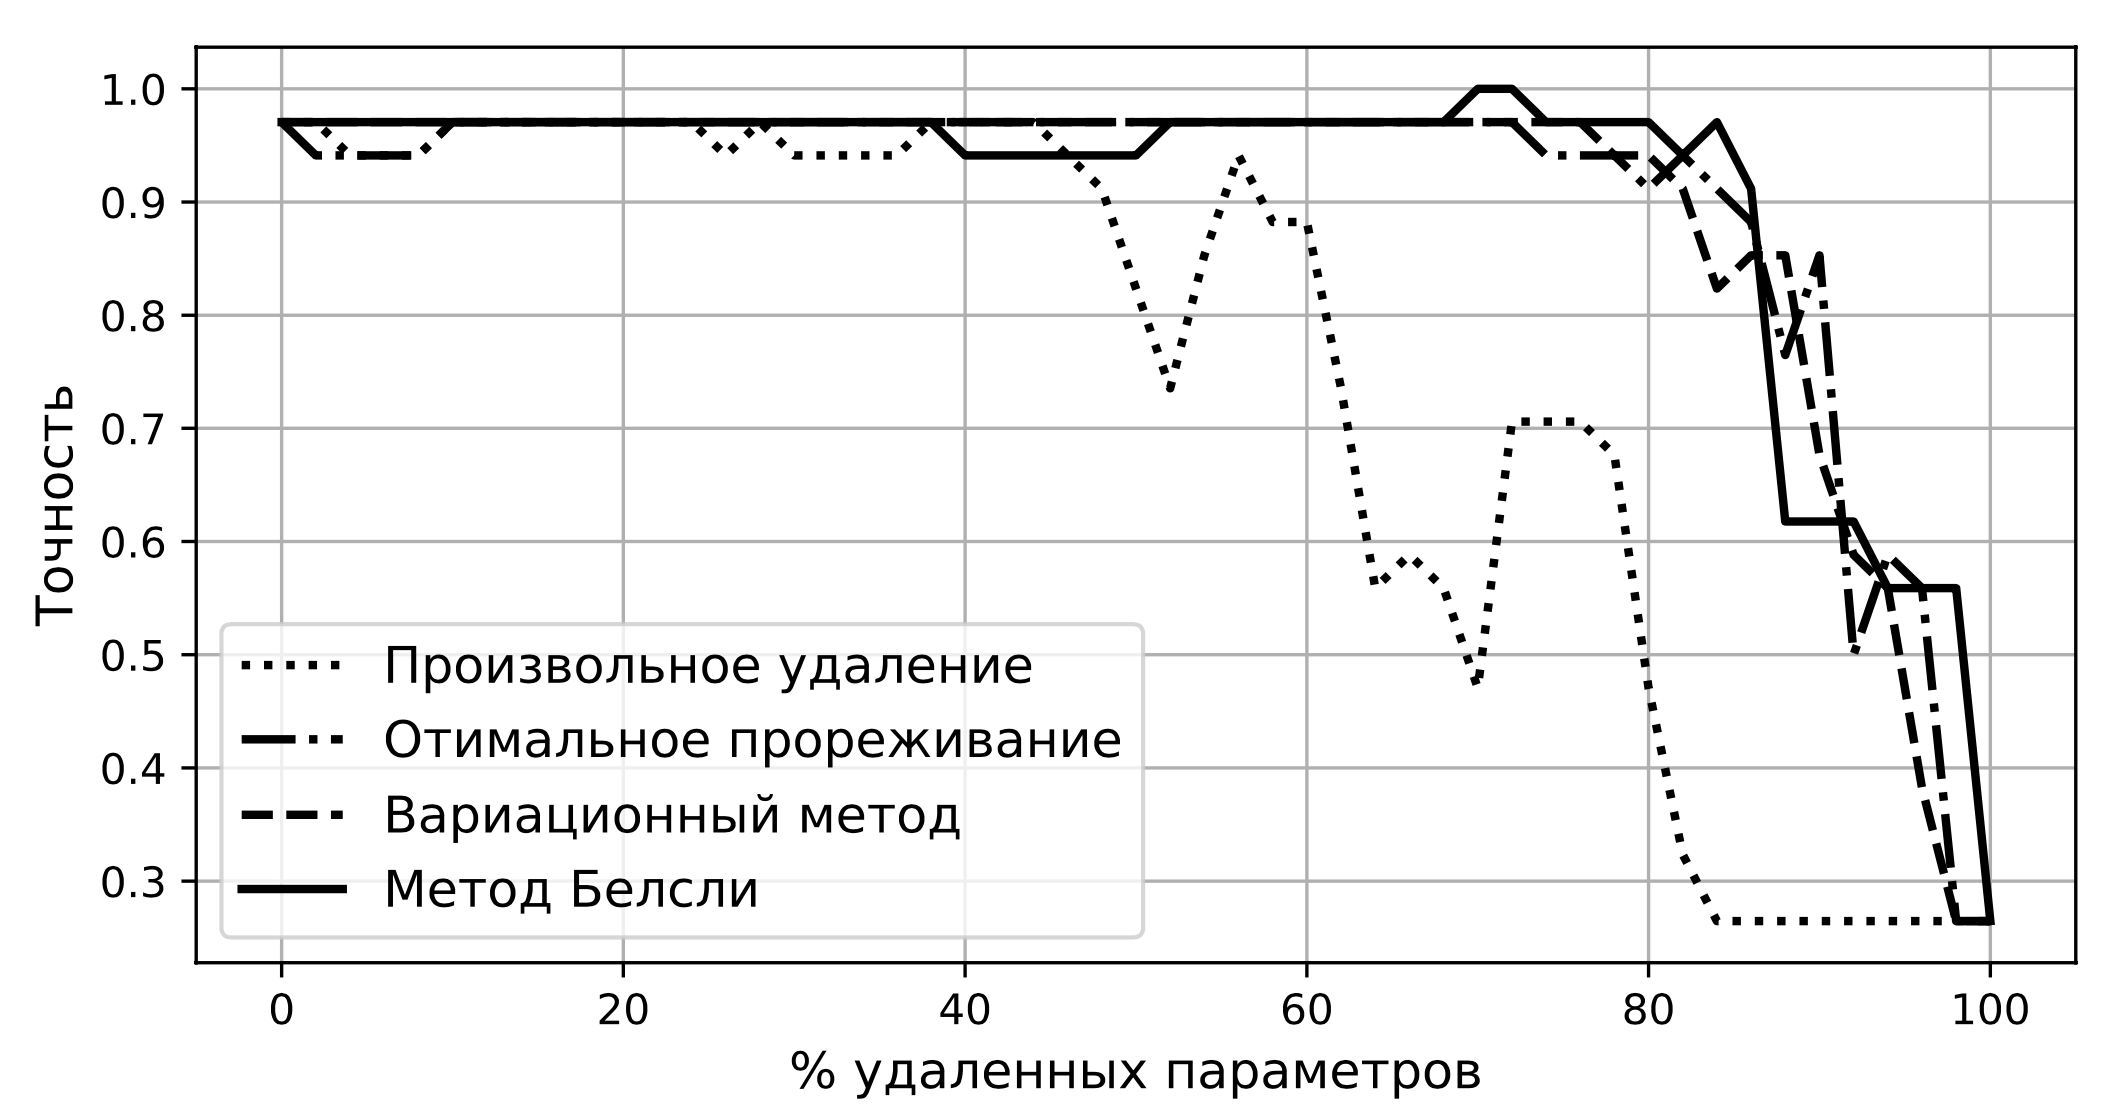
\includegraphics[width=\textwidth]{figures/relevant_class.png}
\end{columns}
\end{frame}

%----------------------------------------------------------------------------------------------------------
\section{Анализ вероятностных свойств ответов модели ученика}
\begin{frame}{Анализ вероятностных свойств ответов модели ученика}
\justifying
~\\[-4mm]
\begin{columns}
\column{0.4\textwidth}
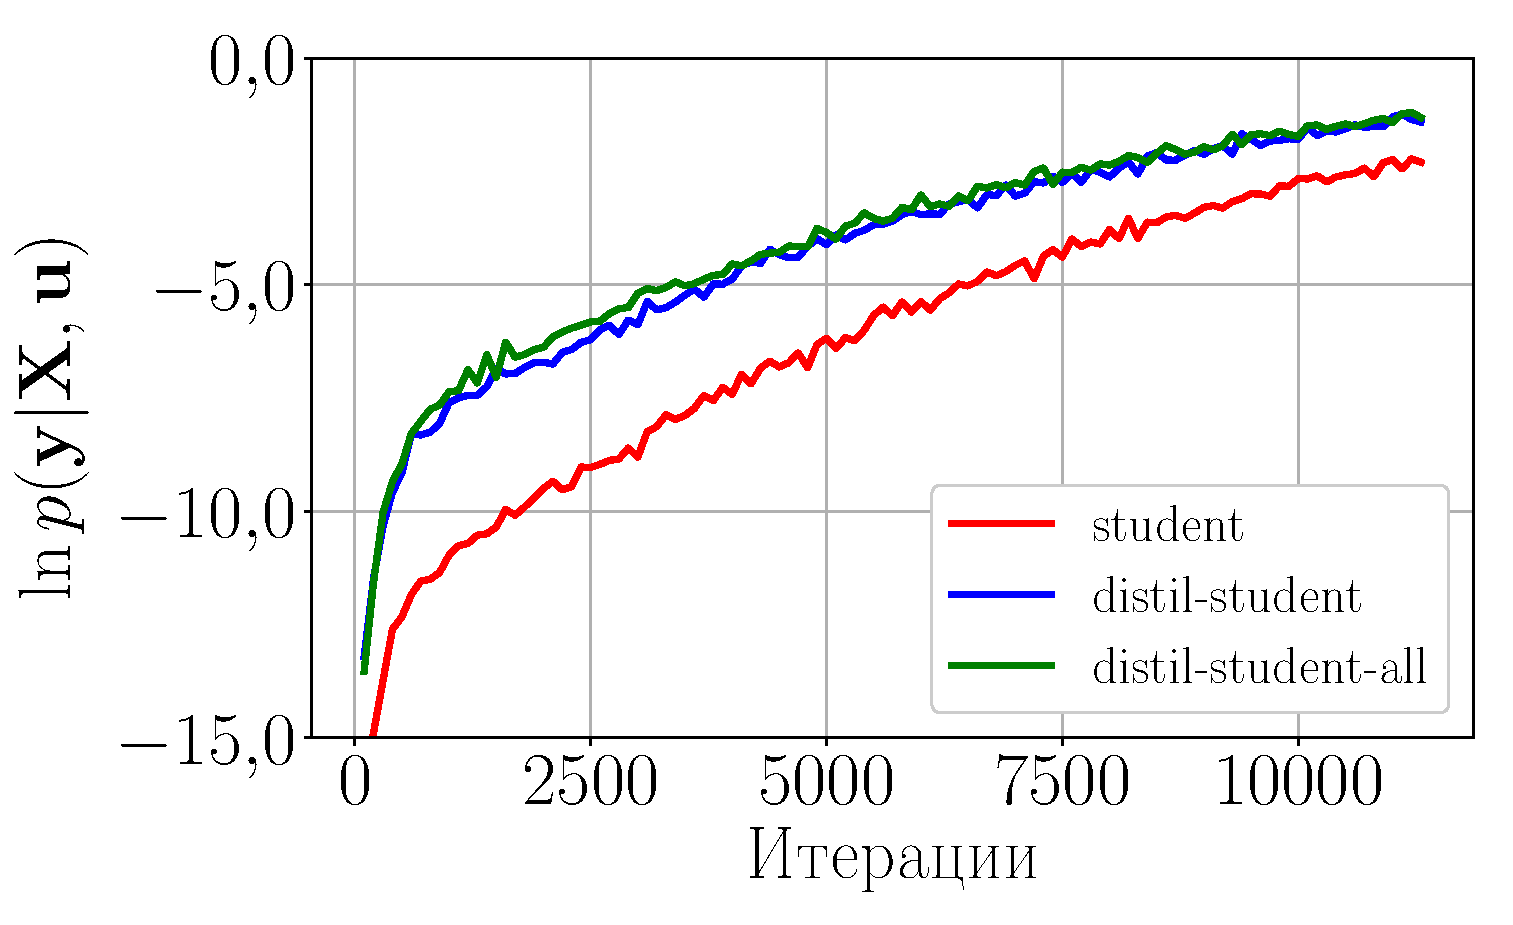
\includegraphics[width=\textwidth]{figures/synthetic_likelihood_2_layers.eps}
\column{0.6\textwidth}

Модель учителя:
$$
\setlength\abovedisplayskip{0pt}
f\bigr(\mathbf{x}\bigr) = \bm{\sigma} \circ \mathbf{U}_3\circ \bm{\sigma} \circ \mathbf{U}_2\circ\bm{\sigma}\circ \mathbf{U}_1\mathbf{x},
\setlength\belowdisplayskip{0pt}
$$
Модель ученика:
$$
\setlength\abovedisplayskip{0pt}
g = \bm{\sigma} \circ \mathbf{W}_2 \circ \bm{\sigma} \circ \mathbf{W}_1, \quad \mathbf{W}_{1} \in \mathbb{R}^{1 \times 50}, \mathbf{W}_{2} \in \mathbb{R}^{50 \times 10}.
\setlength\belowdisplayskip{0pt}
$$
\vspace{-0.8cm}
\begin{table}[]
\begin{center}
\resizebox{\textwidth}{!}{
\begin{tabular}{|l|c|c|c|c|}\cline{1-5}
                  & Учитель           & Без учителя        & Баз. дист. & Байес. дист.\\ \cline{1-5}
Структура            & $[10,100,50,1]$   & $[10,50,1]$       & $[10,50,1]$      & $[10,50,1]$ \\ \cline{1-5}
Числ. парам.    &   6050                       &       550                   &          550               &     550 \\ \cline{1-5}
Инт. метр.    &  -                          &  0                      &  $\mathbf{10244}$             & $\mathbf{25506}$ \\ \cline{1-5}
\end{tabular}
}
\end{center}
\end{table}
\end{columns}

{\emph{Правдоподобие модели ученика на основе {\color{python-green}байесовской дистилляции} растет быстрее чем правдоподобие модели ученика на основе {\color{blue}базовой дистилляции Хинтона}.}}

\vspace{-0.2cm}

\begin{table}[]
\begin{center}
\resizebox{\textwidth}{!}{
\begin{tabular}{|l|c|c|c|c|c|c|}
\hline
\multicolumn{1}{|c|}{Выборка} & Модель      & \begin{tabular}[c]{@{}c@{}}Кросс-энтропийная\\ ошибка\end{tabular} & \begin{tabular}[c]{@{}c@{}}{\color{blue}Кросс-энтропийная} \\ {\color{blue}ошибка с истинными}\\ {\color{blue}вероятностями}\end{tabular} & \begin{tabular}[c]{@{}c@{}}{\color{red}Вероятностная}
\\ {\color{red}разность}\end{tabular} & Точность            & \begin{tabular}[c]{@{}c@{}}Число\\ Параметров\end{tabular} \\ \hline\hline
\multirow{2}{*}{FashionMnist} & с учителем  & $0{,}453\pm0{,}003$                                                & -                                                                                             & $0{,}84\pm0{,}13$                                               & $0{,}842\pm0{,}002$ & 7850                                                       \\ \cline{2-7} 
                              & без учителя & $0{,}461\pm0{,}005$                                                & -                                                                                             & $0{,}86\pm0{,}18$                                               & $0{,}841\pm0{,}002$ & 7850                                                       \\ \hline \hline
\multirow{2}{*}{Synthetic}     & с учителем  & $0{,}618\pm0{,}001$                                                & $\mathbf{1{,}17}\pm\mathbf{0{,}05}$                                                                             & $\mathbf{0{,}45}\pm\mathbf{0{,}20}$                                               & $0{,}828\pm0{,}002$ & 33                                                         \\ \cline{2-7} 
                              & без учителя & $0{,}422\pm0{,}002$                                                & $2{,}64\pm0{,}02$                                                                             & $0{,}75\pm0{,}22$                                               & $0{,}831\pm0{,}001$ & 33                                                         \\ \hline \hline
\multirow{2}{*}{Twitter Sent.}       & с учителем  & $0{,}489\pm0{,}003$                                               & -                                                                                             & $0{,}79\pm0{,}17$                                               & $0{,}764\pm0{,}005$ & 1538                                                       \\ \cline{2-7} 
                              & без учителя &  $0{,}501\pm0{,}006$                                                & -                                                                                             & $0{,}83\pm0{,}22$                                               & $0{,}747\pm0{,}004$ & 1538                                                       \\ \hline 
\end{tabular}
}
\end{center}
\end{table}
{\color{blue}Модель с учителем аппроксимирует истинные вероятности классов.}\\
{\color{red}Модель с учителем имеет меньшую разность между вероятностями классов.}
\end{frame}

%----------------------------------------------------------------------------------------------------------
\section{Выносится на защиту}
\begin{frame}{Выносится на защиту}
\justifying
	\begin{enumerate}
	\justifying
	    \item Предложен байесовский метод выбора моделей с использованием модели учителя с привилегированной и накопленной информацией.
        \item Доказаны теоремы о свойствах дистилляции, 
        \begin{itemize}
            \item[---] \emph{теоремы об эквивалентности} для дистилляции моделей в случае задачи регрессии и классификации,
            \item[---] \emph{теоремы о виде априорного распределения} параметров модели ученика в байесовской дистилляции.
        \end{itemize}
        \item Предложен метод выравнивания структур параметрических моделей. Предложен метод выбора априорного распределения параметров модели ученика с использованием апостериорного распределения параметров модели учителя для случаев
        \begin{itemize}
            \item[---] различных размерностей пространств параметров отдельных слоев,
            \item[---] различного в числа слоев нескольких моделей.
        \end{itemize}
        \item Предложены методы задания порядка на множестве параметров моделей
        \begin{itemize}
            \item[---] на основе корреляции параметров,
            \item[---] на основе оценки скорости сходимости параметров.
        \end{itemize}
        \item Предложена вероятностная интерпретации дистилляции моделей глубокого обучения. Исследованы свойства дистилляции моделей глубокого обучения.
	\end{enumerate}
\end{frame}
%----------------------------------------------------------------------------------------------------------
\section{Список работ автора по теме диссертации}
\begin{frame}{Список работ автора по теме диссертации}
\justifying
{
\scriptsize
\textbf{Публикации в журналах ВАК}

\begin{enumerate}
    \item \textit{Грабовой А.В., Стрижов В.В.} Байесовская дистилляция моделей глубокого обучения~// Автоматика и телемеханика, 2021.
    \item \textit{Грабовой А.В., Стрижов В.В.} Анализ выбора априорного распределения для смеси экспертов~// Журнал вычислительной математики и математической физики, 2021.
    \item \textit{A. Grabovoy, V. Strijov.} Quasi-periodic time series clustering for human // Lobachevskii Journal of Mathematics, 2020.
    \item \textit{Грабовой А.В., Бахтеев О. Ю., Стрижов В.В.} Введение отношения порядка на множестве параметров аппроксимирующих моделей~// Информатика и ее применения, 2020.
    \item \textit{Грабовой А.В., Бахтеев О.Ю., Стрижов В.В.} Определение релевантности параметров нейросети~// Информатика и ее применения, 2019.
    \item \textit{Грабовой А.В., Стрижов В.В.} Вероятностная интерпретация задачи дистилляции~// Автоматика и телемеханика, 2022.
\end{enumerate}

\textbf{Выступления с докладом}
\begin{enumerate}
    \item Задача обучения с экспертом для построения интерпретируемых моделей машинного обучения, Международная конференция <<Интеллектуализация обработки информации>>, 2020.
    \item Привилегированная информация и дистилляция моделей, Всероссийская конференция <<63-я научная конференция МФТИ>>, 2020.
    \item Введение отношения порядка на множестве параметров нейронной сети, Всероссийская конференция <<Математические методы распознавания образов ММРО>>, 2019.
    \item Анализ априорных распределений в задаче смеси экспертов, Всероссийская конференция <<62-я научная конференция МФТИ>>, 2019.
    \item Поиск оптимальной модели при помощи алгоритмов прореживания, Всероссийская конференция <<61-я научная конференция МФТИ>>, 2018.
    \item Автоматическое определение релевантности параметров нейросети, Международная конференция <<Интеллектуализация обработки информации>>, 2018.
\end{enumerate}
}
\end{frame}
%----------------------------------------------------------------------------------------------------------

\end{document} 
